\section{Implementierung}


In diesem Kapitel wird der Aufbau der Applikation veranschaulicht und die implementierten Funktionen und Übergänge der einzelnen Ansichten erklärt. Darüber hinaus wird das verwendete Backend näher betrachtet, bei dem das von Google aufgekaufte Firebase zum Einsatz kommt.
Die Applikation wurde für ein iPhone 7 Plus entwickelt und verfügt daher über keine dynamischen Anpassungen der Darstellungsgrößen für andere Endgeräte.   


\subsection{Anmeldung und Adressbildschirm}
Wird die Applikation das erste mal auf einem Gerät ausgeführt, erscheint der in Abbildung \ref{fig:login_screen} gezeigte \glqq Login Screen\grqq{}. Über den \glqq Sign In\grqq{ }Button kommt der Nutzer zur Registration der Applikation wie es in Abbildung \ref{fig:signin_screen} zu sehen ist.Für die Registrierung und die mit dem Login verbundene Authentifizierung des Nutzers wurden die von Firebase bereitgestellten Lösungen verwendet. Die Anmeldung erfolgt über die Mailadresse eines Google-Kontos.
\newline
Ist das Google-Konto mit der Applikation auf dem iPhone verknüpft, wird dies für die zukünftigen Anmeldungen zwischengespeichert, sodass sich der Nutzer bei einem erneuten Start der Anwendung automatisch am Firebase-Service anmeldet und somit den Login Screen überspringt und direkt in das in Abbildung \ref{fig:address_screen} gezeigte Hauptmenü gelangt.
\begin{figure}[ht]
  \centering
    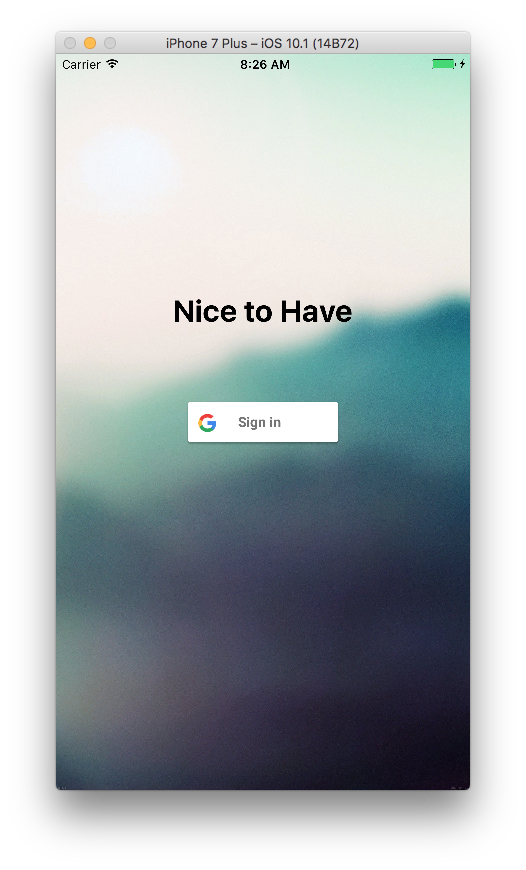
\includegraphics[width=0.3\textwidth]{images/login_screen}
    \caption{Nice to Have - Login Screen}
	 \label{fig:login_screen}
\end{figure}
\newpage
\begin{figure}[ht]
  \centering
    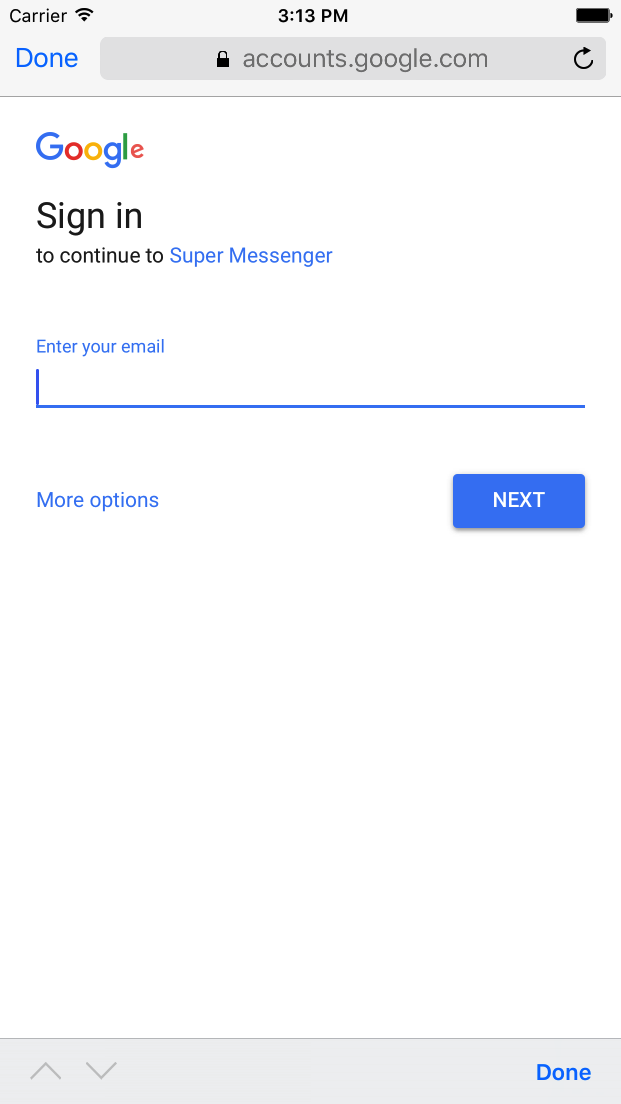
\includegraphics[width=0.3\textwidth]{images/signin_screen}
    \caption{Nice to Have - Anmeldung}
	 \label{fig:signin_screen}
\end{figure}
\begin{figure}[ht]
  \centering
    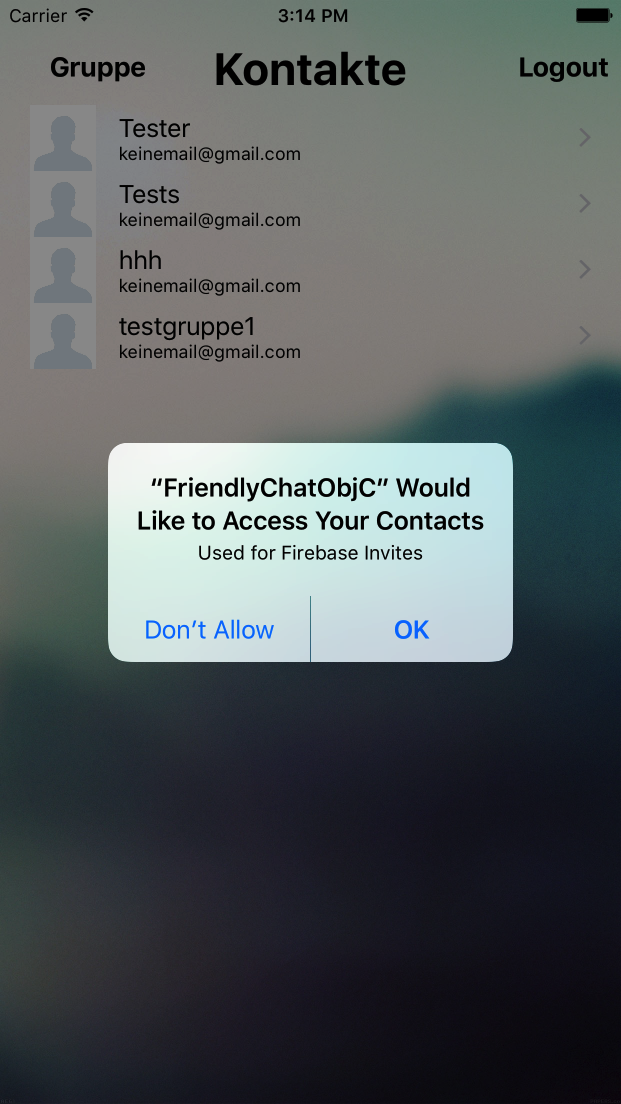
\includegraphics[width=0.3\textwidth]{images/zugriffsabfrage_screen}
    \caption{Nice to Have - Zugriffsabfrage auf das Telefonbuch}
	 \label{fig:zugriffsabfrage_screen}
\end{figure}
\begin{figure}[ht]
  \centering
    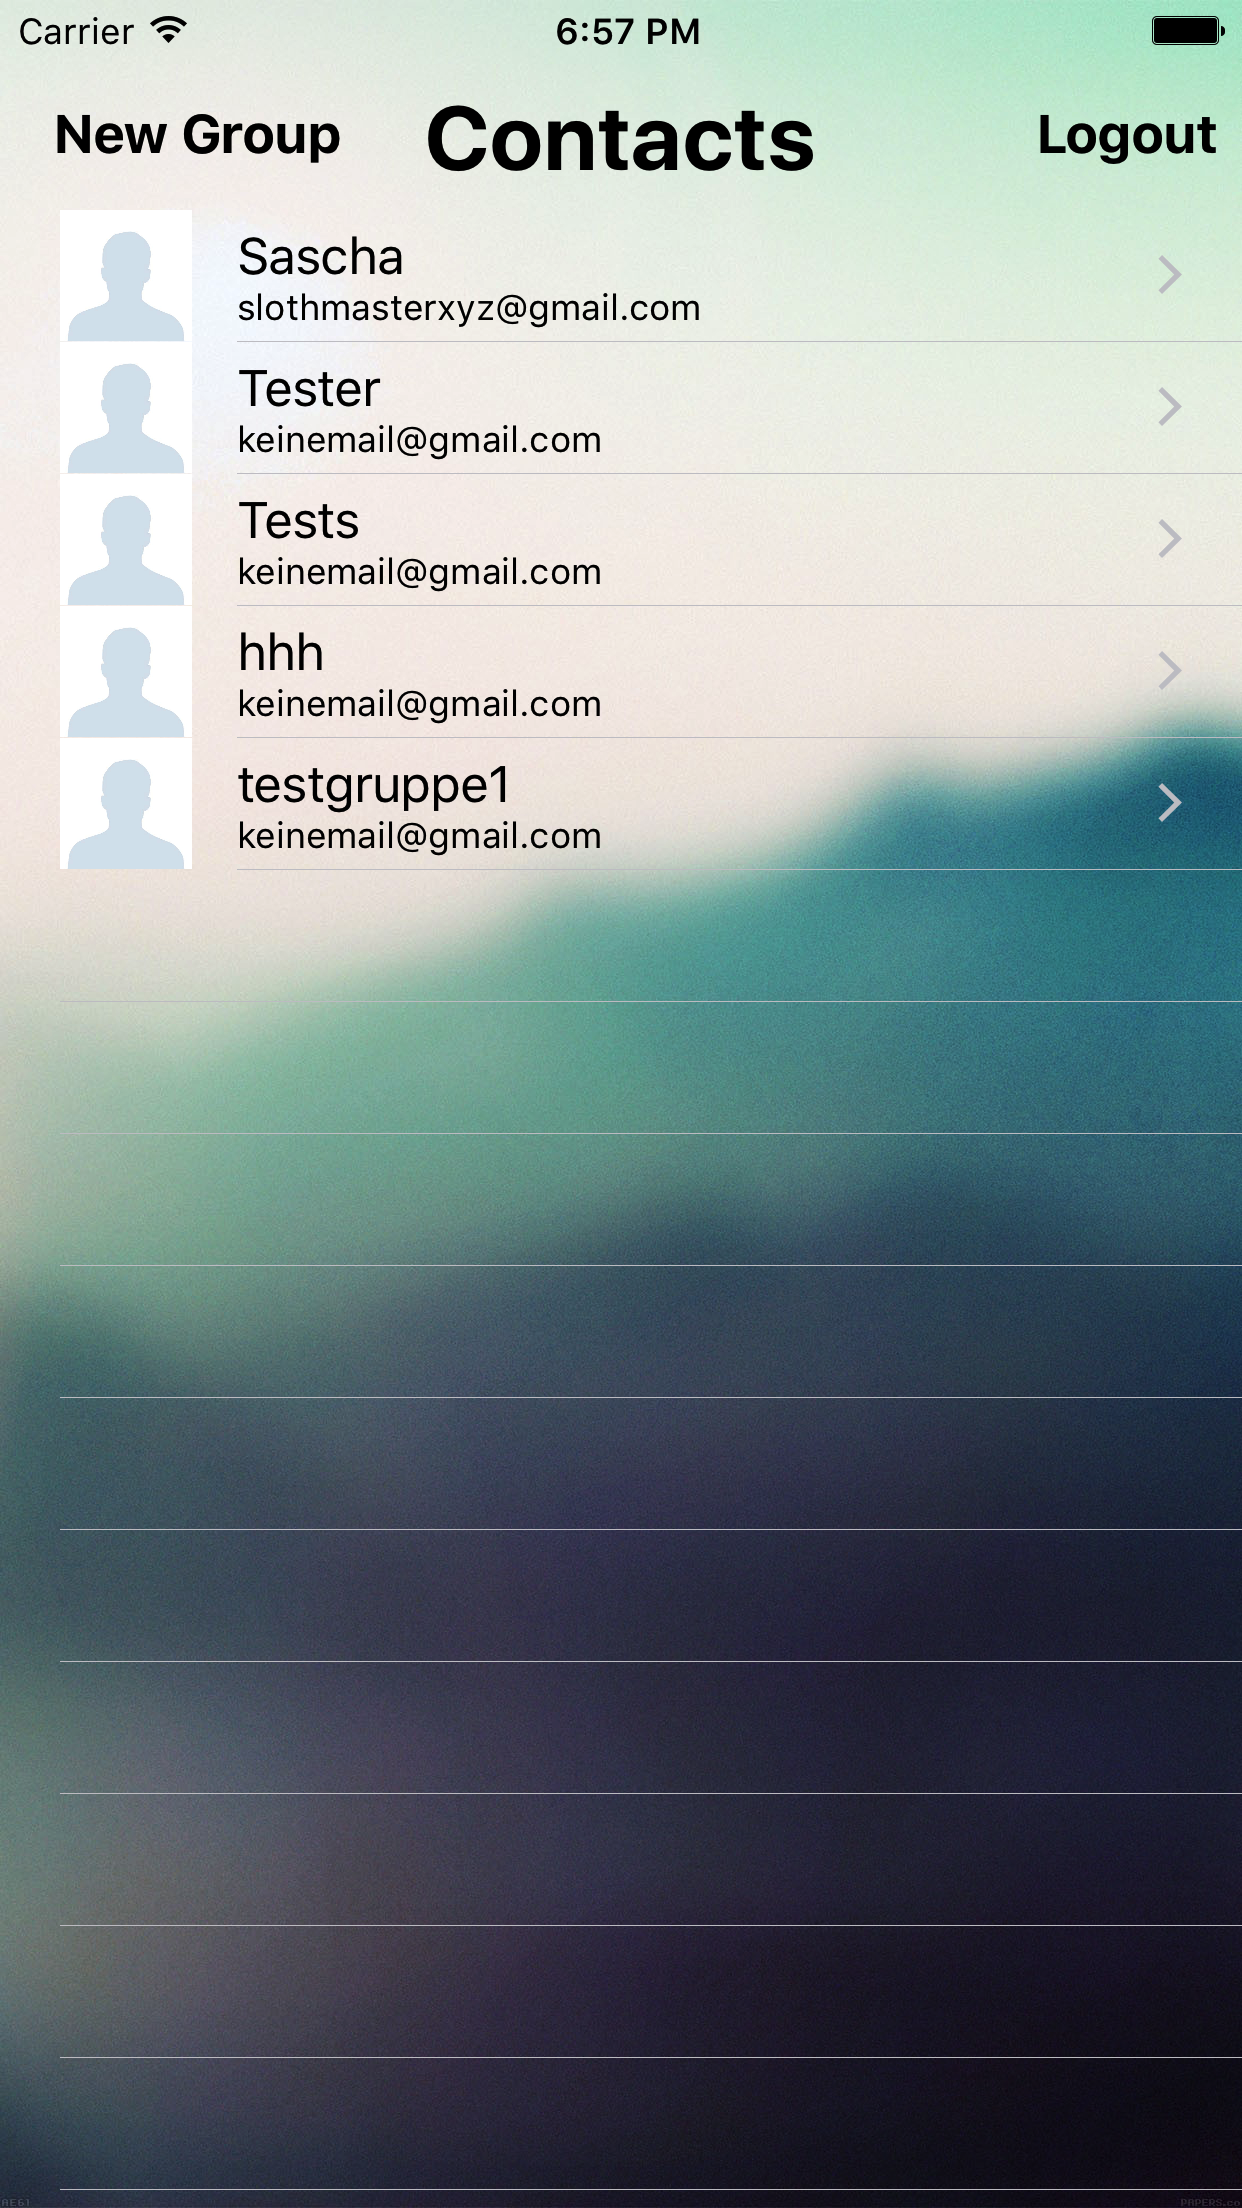
\includegraphics[width=0.3\textwidth]{images/address_screen}
    \caption{Nice to Have - Kontaktliste (Hauptmenü)}
	 \label{fig:address_screen}
\end{figure}
Der Gruppe war es wichtig, ein einheitliches Erscheinungsbild einzuhalten, weshalb das Hintergrundbild des Login Screens für die gesamte Applikation beibehalten wird. Für das Hintergrundbild wurde sich entschieden, weil es nicht zu überladen wirkt und somit der eigentliche Inhalt der Anwendung für die Augen des Benutzers im Vordergrund bleibt. Darüber hinaus hat die helle Erscheinung des Messengers eine offene und nicht ermüdende Wirkung, wie es ein dunkler Hintergrund hätte.
\newline
\newline
Das Hauptmenü erfüllt die Funktionalität einer Kontaktliste. Innerhalb der Kontaktliste werden alle Kontakte angezeigt, welche sich im Adressbuch des Telefons selbst befinden und darüber hinaus die Applikation Nice to Have ebenfalls verwenden. Dies wurde umgesetzt indem zu erst alle Kontakte aus dem Telefonbuch des iPhones auf eine gültige E-Mailadresse von Google untersucht wurden.
Damit jedoch ein Zugriff auf das Adressbuch des Telefons stattfinden kann, muss bei der ersten Verwendung der Applikation der Zugriff auf das Telefonbuch genehmigt werden, welches über die in Abbildung \ref{fig:zugriffsabfrage_screen} gezeigte Abfrage realisiert wird.
Diese Kontakte wurden anschließend anhand ihrer Mailadressen mit den im Backendserver vorhandenen Nutzern vergleichen um festzustellen, ob die gefundenen Kontakte die Applikation ebenfalls verwenden.
\newpage
Für alle Nutzer die sowohl die Applikation verwenden, als auch im Telefonbuch des verwendeten Telefons stehen, wird der entsprechende Kontakt mit Namen und der dazugehörigen Mailadresse in der Kontaktliste angezeigt.
Darüber hinaus wird das für den jeweiligen Kontakt im Telefonbuch des Nutzers hinterlegte Profilbild für die Anzeige verwendet. Sollte ein Kontakt jedoch kein Profilbild im Telefonbuch zugewiesen haben, wird als Alternative ein Bild mit einem hellen Umriss eines Profilbildes angezeigt, um darauf hinzuweisen, dass der angezeigte Kontakt über kein Bild verfügt. Der Gruppe war es wichtig an dieser Stelle der Applikation die Möglichkeit zu haben auf die Bilddateien, welche mit dem Telefonbuch des iPhones verknüpft sind, zuzugreifen und diese darzustellen, anstelle der von Firebase verwendeten Profilbilder des Googleaccounts, wie es innerhalb eines Chats der Fall ist. Dies ermöglicht es nicht nur dem Nutzer der Applikation bestimmten Kontakten individualisierte Bilder zuzuweisen, sondern erleichtert auch die visuelle Verknüpfung eines Kontaktes aus dem Telefonbuch mit dem Kontakt innerhalb der Applikation um diesen leichter wiederzufinden und zu erkennen.
\newpage
\subsection{Gruppenchats}
Neben den Kontakten, welche jeweils eine einzelne Person vertreten, werden ebenfalls Gruppenchats als einzelne Kontakte des in Abbildung \ref{fig:address_screen} gezeigten Hauptmenüs angezeigt. Gruppenchats haben einen eigenen Gruppennamen und bestehen immer aus mindestens zwei beteiligten. Die Implementierung der Gruppenchats erfolgte über eine Liste von den vorhandenen Gruppenchats eines Nutzers, welche von Firebase nach der Authentifizierung an den Nutzer übermittelt wird. Intern werden die Privatchats, welche lediglich zwischen zwei Kontakten geschehen, von den Gruppenchats, bei denen mehrere Kontakte zugleich an einer Konversation teilnehmen können, über eine boolsche Variable mit dem Namen \glqq isprivate\grqq{ }unterschieden.
Über den am rechten oberen Bildschirmrand im Hauptmenü befindlichen Button Logout, kann sich der Nutzer von der Applikation abmelden und gelangt zu dem in Abbildung \ref{fig:login_screen} gezeigten Login Screen zurück.
\newline
\newline
\begin{figure}[ht]
  \centering
    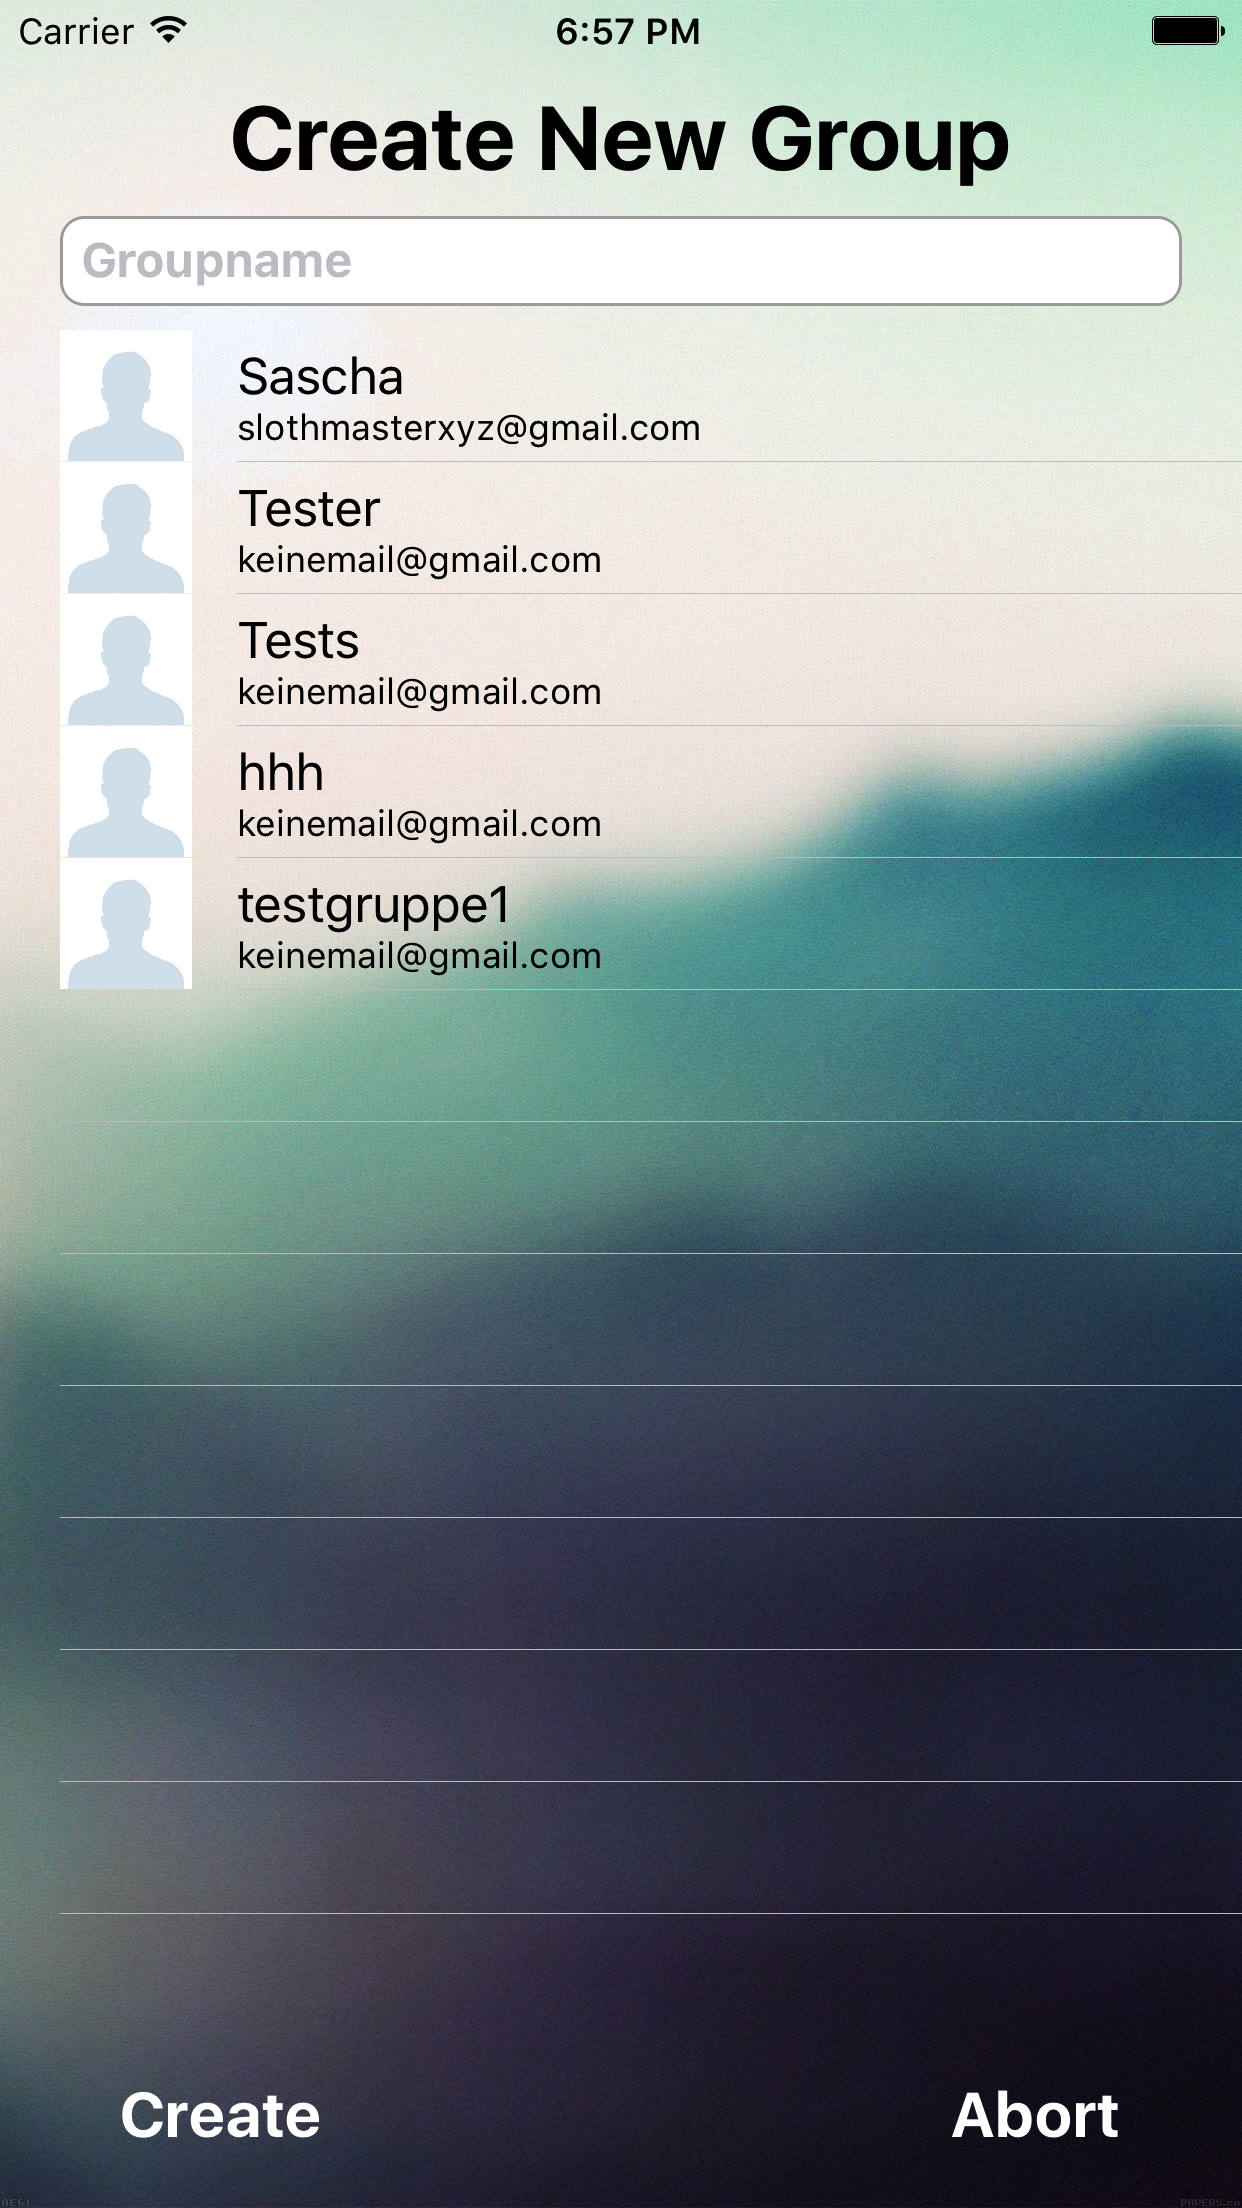
\includegraphics[width=0.3\textwidth]{images/creategroup_screen}
    \caption{Nice to Have - Neue Gruppe erstellen}
	 \label{fig:creategroup_screen}
\end{figure}
Abbildung \ref{fig:creategroup_screen} zeigt den Bildschirm, welcher dem Nutzer angezeigt wird, sobald dieser den im Hauptmenü auf im linken, oberen Bildschirmrand befindlichen Button zum erstellen einer neuen Gruppe auswählt. Beim Erstellen eines neuen Gruppenchats kann der Nutzer den Namen der Gruppe angeben. Dazu wird automatisch, sobald das Eingabefeld für den Gruppennamen ausgewählt wurde, eine Tastatur eingeblendet. Ist der Gruppenname bestimmt, kann der Nutzer die Teilnehmer des Gruppenchats bestimmen, indem über die Kontaktliste beliebig viele Nutzer ausgewählt werden können. Ein ausgewählter Nutzer, welcher der Gruppe hinzugefügt werden soll, wird entsprechend visuell markiert. Sind alle Nutzer, welche dem Gruppenchat hinzugefügt werden sollen ausgewählt, kann der Nutzer die Erstellung der Gruppe abschließen und auf den \glqq Create\grqq{-}Button drücken oder die Aktion über den \glqq Abort\grqq{-}Button verwerfen. Sobald eine der beiden Möglichkeiten ausgewählt wurde, gelangt der Nutzer zurück in das in Abbildung \ref{fig:address_screen} gezeigte Hauptmenü.
\newpage
\subsection{Chatfenster}
Wählt der Nutzer einen Kontakt im Hauptmenü aus, so öffnet sich je nach dem ob es sich bei dem Kontakt um eine Gruppe oder eine einzelne Person handelt, der entsprechende Chat wie es in Abbildung \ref{fig:chat_screen} zu sehen ist. Die einzelnen Chats werden über einzigartige Kennzeichnung (identifier) angesteuert. Jeder Chat bekommt von Firebase eine solche einzigartige Kennzeichnung zugewiesen, über die ein Client den gewünschten Chat anfordern kann. Die einzige Bedingung welche überprüft wird ist, ob der Nutzer ein Teilnehmer des angeforderten Chats ist.
\newline
\newline
Innerhalb des Chatfensters werden eigene Nachrichten mit einer dunklen Sprechblase dargestellt. Nachrichten von anderen Teilnehmern des Chats werden mit einer helleren Sprechblase angezeigt. Dies soll besonders das native Verständnis des Nutzers fördern, welche Nachrichten von einem selbst und welche von anderen Teilnehmern verfasst wurden sind. Dies unterstützt vor allem die Fähigkeit, einen schnellen Überblick über den Chatverlauf zu erlangen, sobald man einen Chat öffnet, welcher bereits eine vergangene Konversation enthält. Dies wird ebenfalls dadurch unterstützt, dass die eigenen Nachrichten neben der unterschiedlichen Farbe der Sprechblase, immer auf dem Display von der rechten Seite aus erscheinen, wobei Nachrichten von anderen Teilnehmern immer von der linken Seite aus angezeigt werden. Innerhalb einer jeden Sprechblase befindet sich der Name des Verfassers der Nachricht, um eine geeignete Zuordnung der Nachrichten im Schriftverkehr mit mehreren Teilnehmern zu ermöglichen. Ebenfalls ist innerhalb einer Sprechblase das Datum und die Uhrzeit der zu sehen, zu der die Nachricht von dem Nutzer versendet wurde.
\begin{figure}[ht]
  \centering
    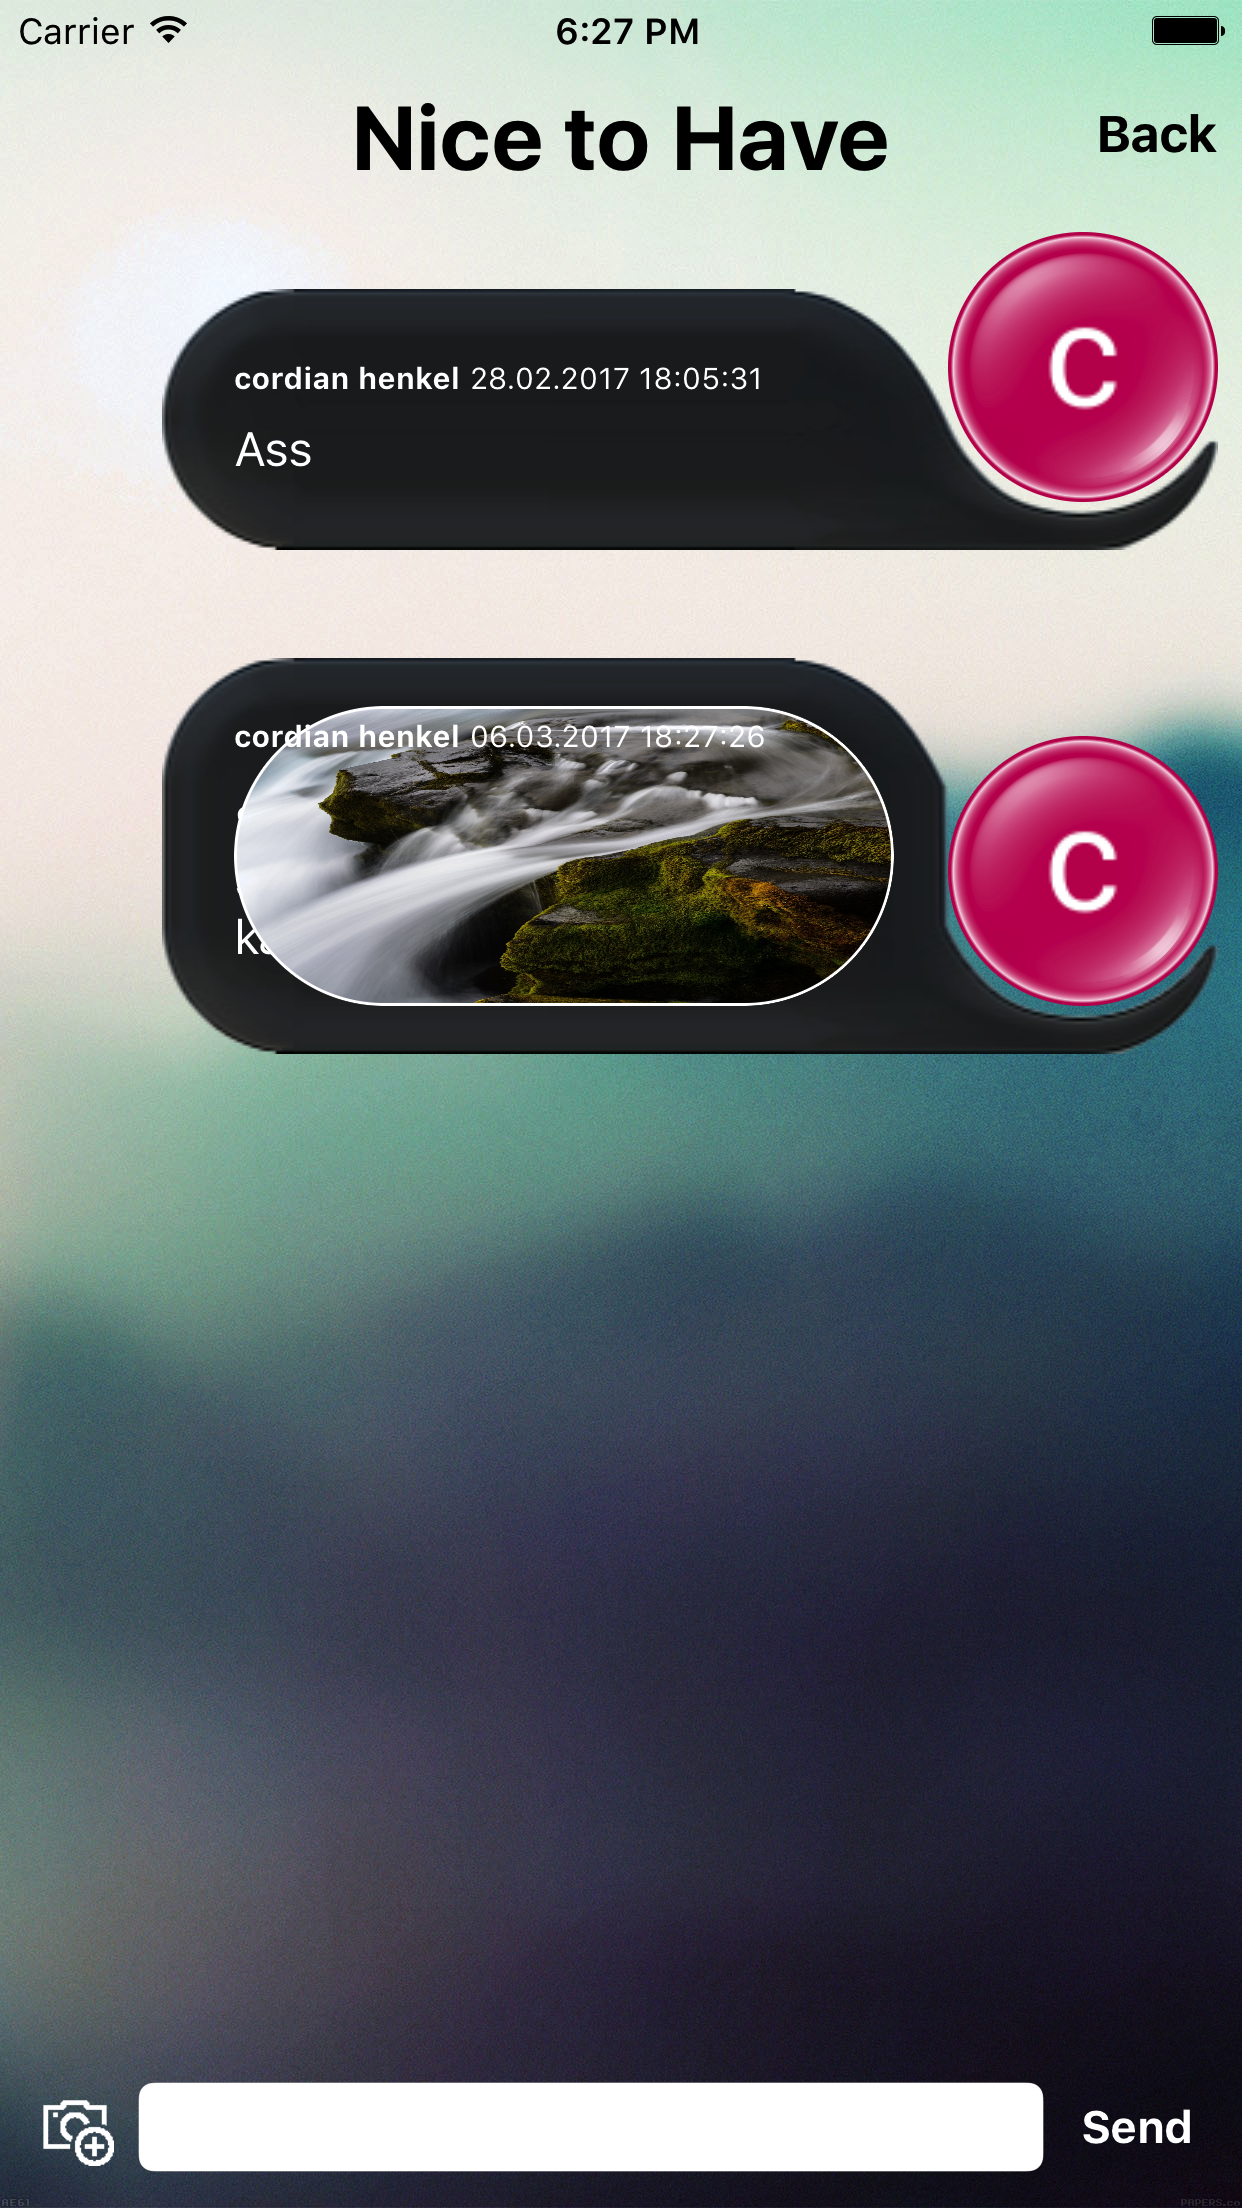
\includegraphics[width=0.3\textwidth]{images/chat_screen}
    \caption{Nice to Have - Chatfenster}
	 \label{fig:chat_screen}
\end{figure}
Im Gegensatz zur Kontaktliste im Hauptmenü, wird für den Avatar eines Chatteilnehmers das bei dem verwendeten Googleaccount hinterlegte Profilbild verwendet. Dies ermöglicht es den Chatteilnehmern ihre Erscheinung nach außen zu anderen Teilnehmern der Applikation zu individualisieren und anzupassen. Eine visuelle Verbesserung der Bilder für die Avatare der einzelnen Chatteilnehmer sorgt ein Hochglanzeffekt, welcher durch ein transparentes Bild mit einem weißen Schimmer an den Rändern realisiert wird.
\newline
\newline
Eine wichtige Voraussetzung für einen komplikationslosen Umgang mit der Applikation war es, die Eingabemaske und die bereits empfangenen Nachrichten entsprechend neu zu positionieren, sobald die Tastatur zum schreiben einer neuen Nachricht eingeblendet wurde. Die Tastatur wird automatisch von unten in den Bildschirm eingefahren, sobald der Nutzer das Eingabefeld am unteren Bildschirmrand anwählt. Die Größe der Tastatur ist abhängig vom Modell des Telefons, weshalb die Ansicht nicht um einen statischen Wert angepasst werden kann. Deshalb wird abhängig von der Tastaturgröße, die gesamte View, auf der sich die Eingabemaske und die bereits empfangenen Chatnachrichten befinden, nach oben verschoben.
Wird die Textnachricht abgeschickt, indem der Nutzer auf den \glqq Senden\grqq{-}Button drückt, wird die Tastatur eingefahren und verschwindet vom Bildschirm. Mittels eines Events, welches dabei ausgelöst wird, wird die View erneut um die dynamische Größe der Tastatur angepasst und nach unten verschoben.
Ebenfalls war es wichtig, wie man die Tastatur einfährt, ohne eine Nachricht abzuschicken, da sich hierfür keine Taste mit entsprechender Funktion auf der eingeblendeten Tastatur befindet. Um dies zu realisieren, wird dem Textfeld der sogenannte \glqq first responder\grqq{ }entzogen, sobald der Nutzer den Chat und somit etwas außerhalb der Tastatur auswählt.
\newline
Verwendet der Nutzer den \glqq Back\grqq{-}Button im oberen rechten Teil des Bildschirms gelangt dieser zurück zum Hauptmenü von Abbildung \ref{fig:address_screen}.
\newpage
\subsection{Bilder}
Neben dem austauschen von Textnachrichten ist es möglich, Bilder an andere Chatteilnehmer zu versenden. Wählt ein Nutzer das Kamerasymbol am linken unteren Bildschirmrand des in Abbildung \ref{fig:chat_screen} gezeigten Chatfensters aus, öffnet sich eine Übersicht von den verschiedenen Fotoalben des Nutzers wie es in Abbildung \ref{fig:sendphotos_screen} zu sehen ist. Über diese Ansicht kann der Nutzer Bilder, welche lokal auf dem Handy gespeichert sind auswählen und diese mit den Chatpartner oder der gesamten Gruppe teilen. Über den \glqq Cancel\grqq{-}Button im oberen rechten Bildschirmrand kann die Aktion abgebrochen werden und der Nutzer gelangt zurück zum Chatfenster.
\begin{figure}[ht]
  \centering
    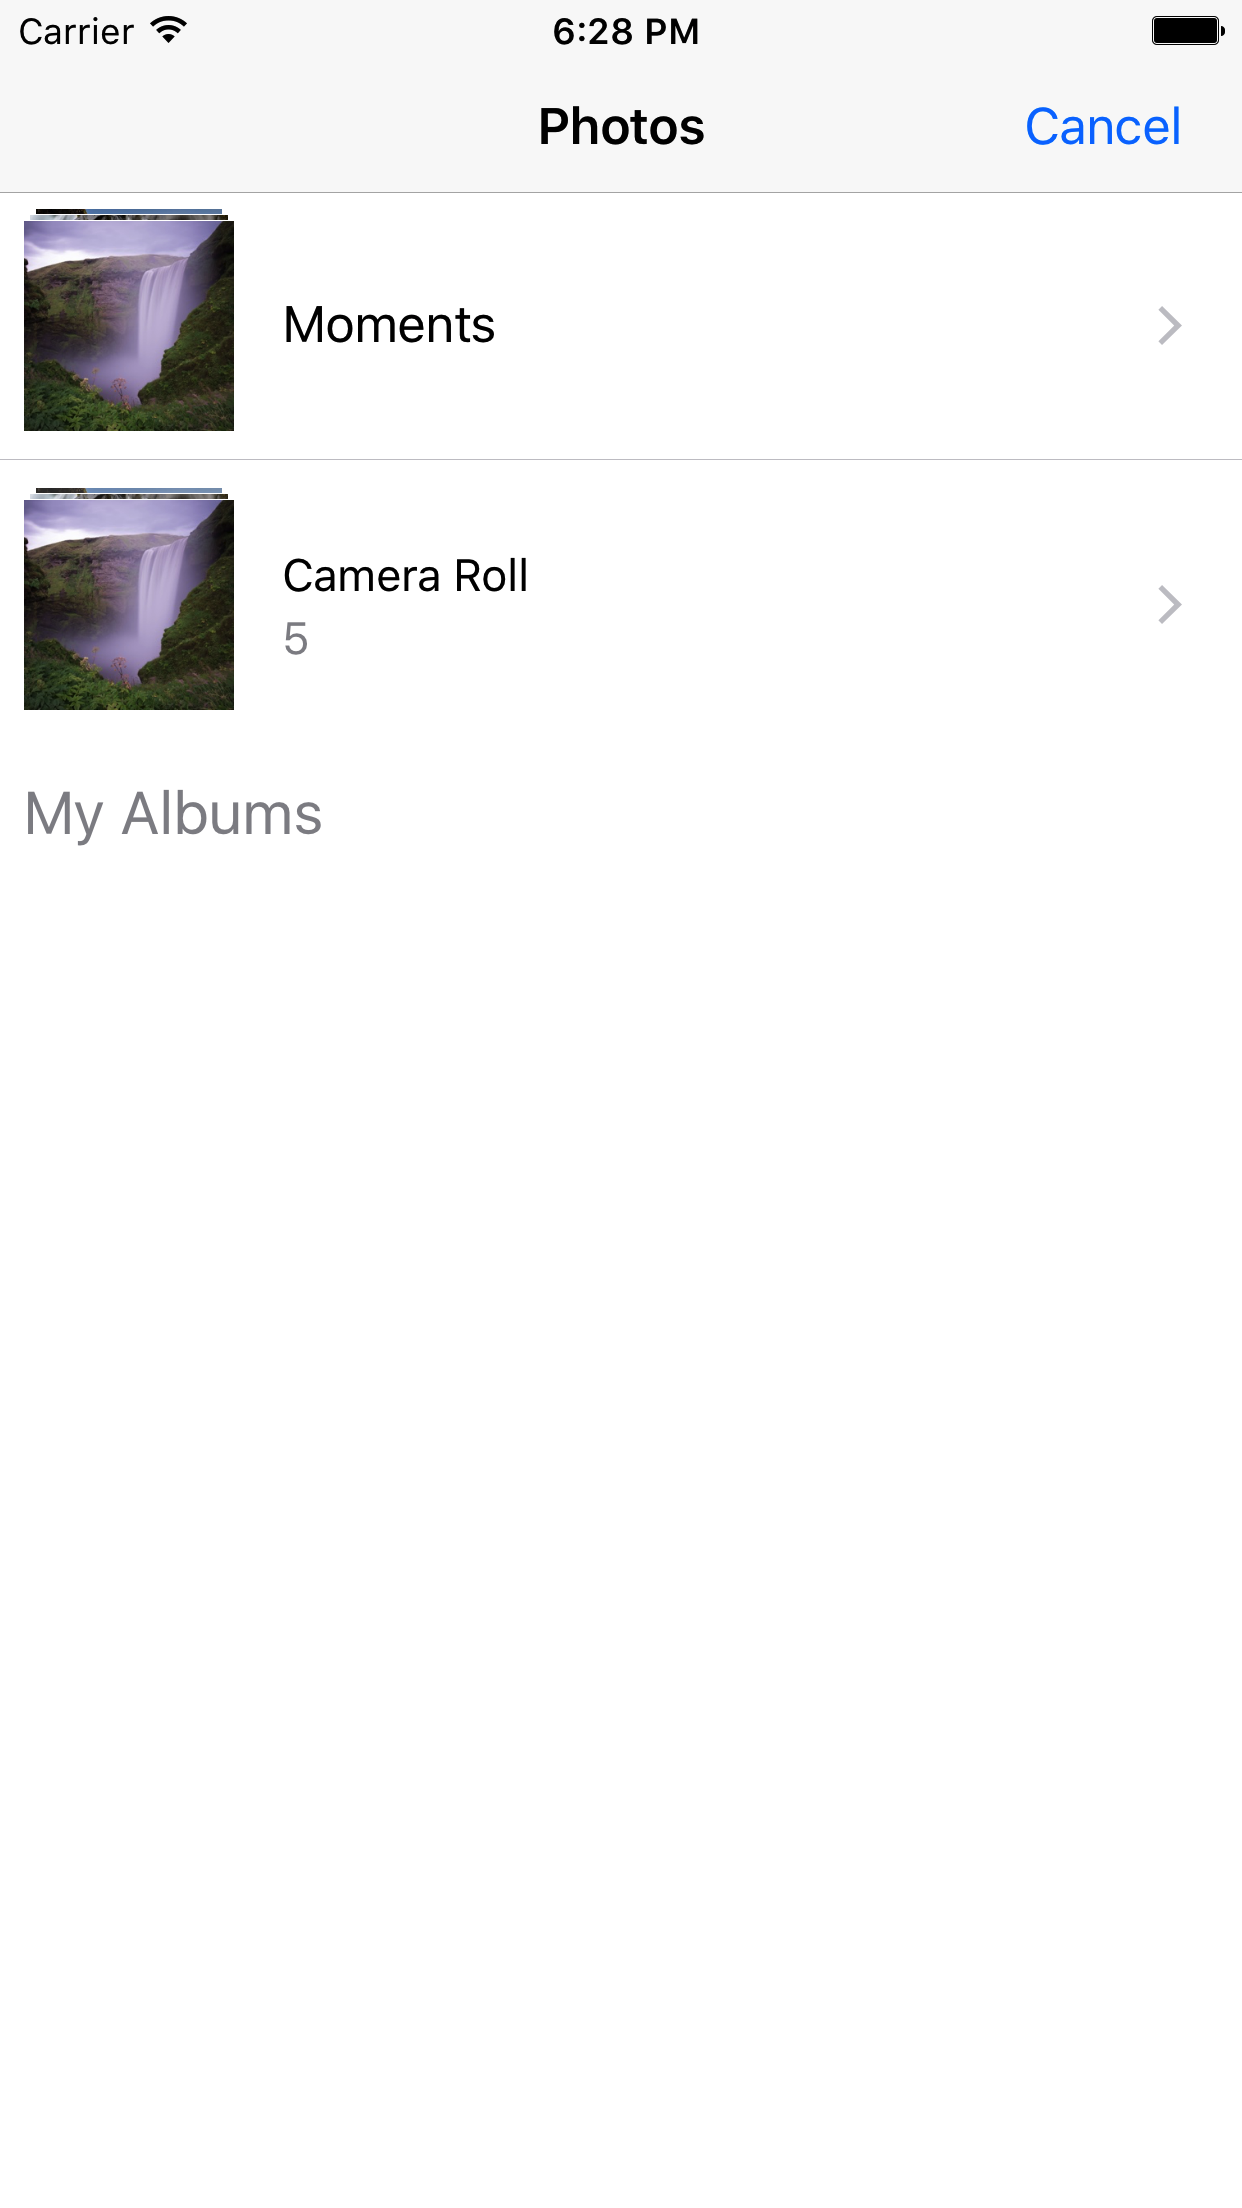
\includegraphics[width=0.3\textwidth]{images/sendphotos_screen}
    \caption{Nice to Have - Senden von Bildern}
	 \label{fig:sendphotos_screen}
\end{figure}
\newpage

\subsection{Backend}



% \begin{figure}
 % \centering
 %   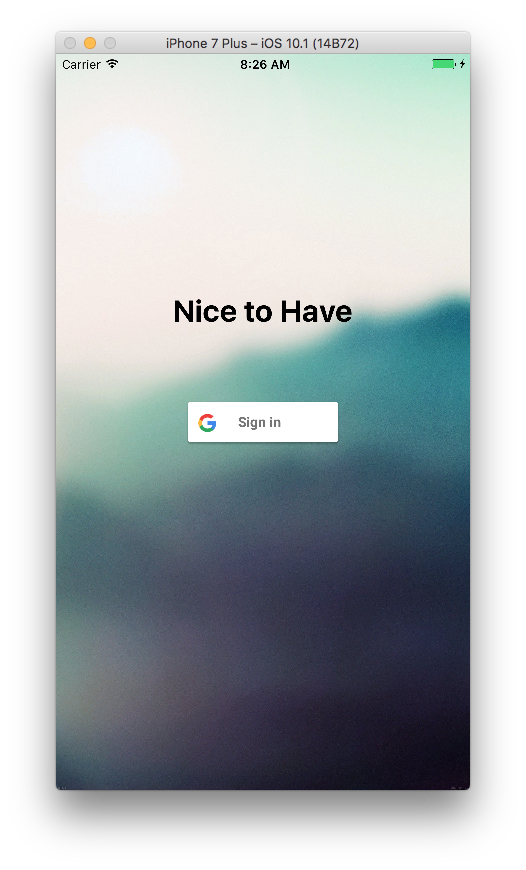
\includegraphics[width=0.3\textwidth]{images/login_screen}
 %   \caption{Nice to Have - Login Screen}
 % \label{fig:login_screen}
%\end{figure}